\chapter{Frontend}
\section{Ideensammlung}
In diesem Teil finden alle Ideen und Gedanken zu dem Projekt Platz welche ich vor Projektbeginn hatte.
\subsection{Allgemeine Ideen}
\paragraph{Partikeleffekte}
\mbox{}\\
Bei Kollision des Balles mit den Wänden, den Schlägern oder gar anderen Bällen wäre ein Partikeleffekt sehr schön.
\newline
Ebenfalls könnte man mit Partikeleffekten den Ballverlust (Zerstörung des Balles in den "Toren") sehr schön grafisch unterstreichen.
\newline
Möglicherweise dafür geeignete Engine:
\href{http://soulwire.github.io/sketch.js/}{Sketch.js}
\paragraph{Multiplayer}
\mbox{}\\
Ideen zu Spielen mit mehr als 2 Spielern.
\begin{itemize}
	\item Punkt bei Ballverlust erhält der letzte Spieler. Spiel merkt sich letzte 2 Ballkontakte sodass der Abschläger erkannt werden kann.
	\item Spieler \& Ball färben. Man könnte die Schläger Färben und die Bälle bei Ballkontakt der eigenen Farbe zuweisen. So erhalten die Spieler einen Visuellen Indikator wer Punkte bekommen kann.
\end{itemize}
\newpage
\paragraph{Schläger}
\begin{itemize}
\item
\textbf{Bewegung des Schlägers} Bewegung kann Relativ oder Absolut erfolgen. Bei absoluter Bewegung wird der Schläger sehr stark springen und möglicherweise das Spiel zu einfach werden.
\item
\textbf{Geschwindigkeit} Man sollte die Geschwindigkeit des Schläger begrenzen sodass das Spiel  schwieriger wird.
\item
\textbf{Begrenzung} Der Schläger braucht 2 Begrenzungen damit er das Spielfeld nicht verlässt.
\item
\textbf{Input der Controller} Der Input sollte so einfach wie möglich gestaltet werden. Am besten nur die Richtung und die Positionsänderung übertragen.
\end{itemize}
\subsection{Spielfelder}
\paragraph{Original Pong}
\mbox{}\\
Im Orinalen Pong betrugen die Abmaße der Komponenten folgende werte:
\begin{itemize}
	\item
	      Spielfeld Größe: 512*256px
	\item
	      Ball 6*5px
	\item
	      Schläger 2*28px
	\item
	      Schläger Geschwindigkeit 4px pro Intervall
\end{itemize}
\newpage
\paragraph{2 Spieler Normal}
\mbox{}\\
\begin{figure}[ht]
	\begin{center}
		\makebox[\textwidth]{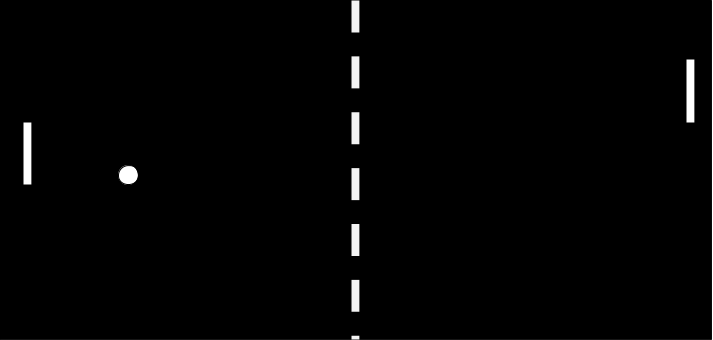
\includegraphics[width=300pt]{frontend/Ping-Pong-2p.png}}
	\end{center}
	\caption{Mockup eines 2-Spieler Feldes}
	\label{figx}
\end{figure}
\newline
\paragraph{2 Spieler Breakout}
\mbox{}\\
Die Idee für dieses Feld war es 2 Klassiker miteinander zu verbinden. Die Spieler zerstören mit einem eigenen Ball die Felder. Das Spiel endet wenn alle Felder zerstört sind. Gewinner ist der Spieler welcher mehr Felder zerstört hat.
\newline
Die Spieler sollten nur den eigenen Ball beeinflussen können. Also muss für den jeweils anderen Spieler eine Barriere errichtet werden.
\newline
\begin{figure}[ht]
	\begin{center}
		\makebox[\textwidth]{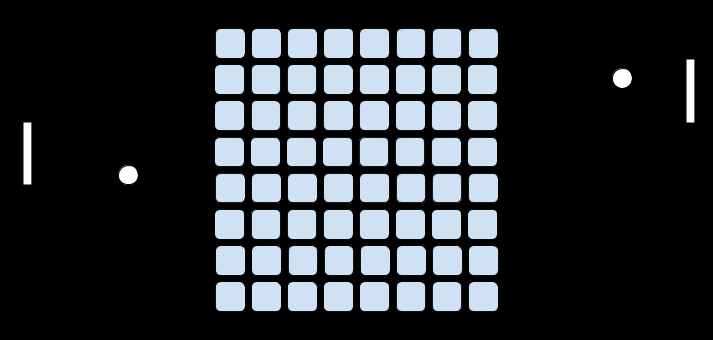
\includegraphics[width=300pt]{frontend/Ping-Pong-Breakout.png}}
	\end{center}
	\caption{Mockup eines 2-Spieler Feldes im Spielmodus Breakout}
	\label{figx}
\end{figure}
\newpage
\paragraph{3 Spieler}
\mbox{}\\
Als ich die Präsentation des Projektes sah war ich nicht mit den Ideen für einen Multispielermodus zufrieden. Sofort kam mir folgende Idee:
\newline
3 Spieler spielen in einem abgeschnittenem Dreieck, bzw eines gleichseitigen Sechseckes. Jeder kontrolliert eine Seite.
\newline
\begin{figure}[ht]
	\begin{center}
		\makebox[\textwidth]{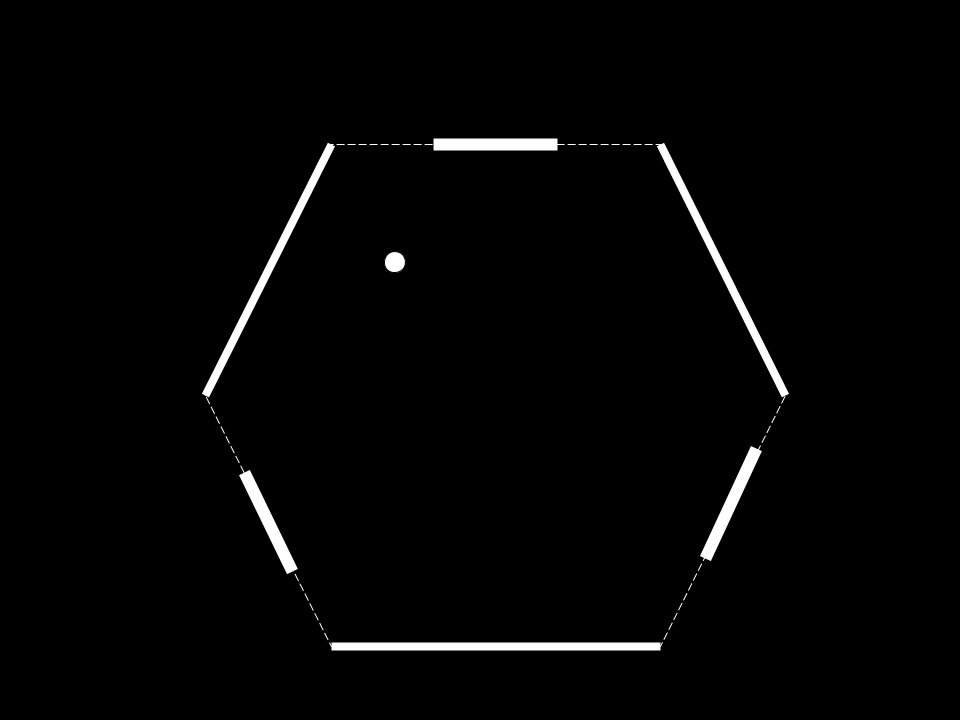
\includegraphics[width=300pt]{frontend/Ping-Pong-3p.png}}
	\end{center}
	\caption{Mockup eines 3-Spieler Feldes}
	\label{figx}
\end{figure}
\newline
\paragraph{4 Spieler}
\mbox{}\\
Als weitere Idee kam mir ein Vier-Spieler Feld bei dem sich in einem Quadrat je 2 Spieler gegenüberstehen.
\newline
Mehr als 4 Spieler sind meiner Meinung nach nicht notwendig. Wenn man bedenkt das sich die Spieler vor einem Bildschirm im Flur sammeln.
\newline
Denkbar ist allerdings das man das Konzept für 3 und 4 Spieler für weitere Spieler weiterführt.
\newpage
\subsection{Power-Ups}
Kurze Ideensammlung zu möglichen Verstärkungen.
\begin{itemize}
	\item
	      \textbf{Magnet:} Ball wird vom Schläger angezogen. Der Spieler erhält dann die Möglichkeit den Ball zu führen und gezielt abzustoßen.
	\item
	      \textbf{Größerer / Kleinerer Ball:} Ball-Modifikator, denkbar auch eine pulsierende Variante wobei sich der Ball durchgehend in der Größe verändert.
	\item
	      \textbf{Multi-Ball:} Ball wir mehrfach dupliziert. Die verschiedenen Bälle fliegen vom Startpunkt aus in alle Richtungen und zählen alle als normaler Ball. Bei Ballverlust tauchen diese nicht erneut auf.
	\item
	      \textbf{Steuerung Invertieren:} Steuerung des Gegners wird invertiert.
	\item
	      \textbf{Geschwindigkeitsmodifikation des Schlägers:} Eigener Schläger wird schneller oder gegnerischer wird langsamer.
\end{itemize}
\subsection{Statistiken}
Auflistung an Daten welche für eine Statistik relevant wären.
\begin{itemize}
	\item
	      Spieldauer
	\item
	      Ballkontakte je Spieler
	\item
	      Zurückgelegte Distanz des Balles
	\item
	      Zurückgelegte Distanz je Spieler
	\item
	      Genauigkeit der Schläger
	      \newline
	      (Ballkontakte / Durchgelassene Bälle)
\end{itemize}
\newpage
\section{Auswahl einer Physics-Engine}

\begin{quote}
	\href{https://github.com/Transport-Protocol/MBC-Ping-Pong/issues/3}{Auswahl einer geeigneten 2D-/Physiksengine \#3}
	\newline
	Die Darstellung auf dem Anzeigegerät ist über den DOM nicht möglich, da die Bewegung des Balls und der Schläger zu schnell werden. Zudem wird auch die Physik auf dem Anzeigegeräts berechnet. Hierfür ist eine Kollisionserkennung erforderlich.
\end{quote}
Für die physikalisch korrekte Kollision des Balles mit der Spielwelt und den Schlägern haben wir uns entschieden eine Physics-Engine zu verwenden.

\subsection{Matter.JS}
Matter js ist eine sehr mächtige Engine. Sie unterstützt viele Formen und Physikalische Eigenschaften wie zum Beispiel Masse und wirkende Kräfte auf die jeweiligen Objekte. 
Es besteht die Möglichkeit physikalische Objekte zusammen zusetzen und sogar diese Elastisch erscheinen zu lassen, so ist es beispielsweise möglich Stoff oder schwingende Seile zu erstellen.
Nach mehrstündiger Einarbeitung kam ich zu dem Schluss das diese Engine für unser Projekt nicht geeignet ist.
Gründe hierfür sind:
\begin{itemize}
	\item
	      Zu Komplex:
	      Die Einrichtung des Spielfeldes erwies sich als überaus schwierig. Gute Anleitungen für einfache Szenarien fehlten, die verfügbaren Anleitungen sind zu grundlegend beschrieben.
	      Ebenfalls half die Anleitung der Engine nicht bei der Verwendung der einzelnen Komponenten.
	\item
	      Die Positionierung der Objekte bezog sich immer auf den Mittelpunkt des Objektes, man kann beispielsweise kein Rechteck von (x,y) nach (x1,y1) erstellen sondern muss den Mittelpunkt und die Abmaße des Objektes angeben.
	\item
	      Physik nicht immer korrekt. Die Engine sollte den Ball richtig von einer Ebene abprallen lassen, diese Engine allerdings lies den Ball teilweise an Plattformen abrollen obwohl keine Schwerkraft vorhanden war. Ich schließe darauf das die Engine Reibungskräfte und vielleicht sogar Anziehungskräfte zwischen den Objekten herstellt. Für unser Projekt ist dies aber nicht zu gebrauchen.
	\item
	      Schwer zu debuggen. Während meiner Versuche bin ich immer wieder auf Probleme gestoßen. Einige der Debugausgaben ließen sich gut ableiten und waren hilfreich. 
	      Allerdings bin ich auch auf einige Probleme gestoßen welche nicht in den Debugausgaben behandelt wurde. Meine letzten Versuche endeten alle darin das der Browser gecrasht ist aufgrund eines Memory-leaks.
\end{itemize}
\subsection{Phaser.io}
Phaser.io beschreibt sich selber als html5 Game Framework. Es wurde nach dem mobile-first Prinzip entwickelt und ist opensource.
Die Entwicklung des gewünschten Prototypen erwies sich als sehr leicht, da es viele gute Beispiele gibt.
Die Engine unterstützt von Haus aus eine Arcade-Physic, diese ist perfekt für unser Projekt. Sie beinhaltet Kollisions und Bewegungsfunktionen für den 2-Dimensionalen Raum
\subsection{Erstellung eines Prototypen}
In Phaser erstellt man ein Spiel über den Aufruf 'new Phaser.Game(...) die ersten Beiden Argumente geben die Dimensionen des Spielfeldes an, also die Weite und Höhe in Pixeln. 
\newline
Der Nächste Parameter bestimmt die Render-Engine. 
Mögliche Werte sind 'Phaser.CANVAS', 'Phaser.WEBGL' oder 'Phaser.AUTO', wenn 'Phaser.AUTO' verwendet wird so probiert die Engine erst WebGL aus und für den Fall das der Browser WebGL nicht unterstützt wird Canvas verwendet.
\newline
Das nächste Argument gibt das Ziel im DOM an, wenn man diesen Parameter nicht setzt wird das Spiel einfach im Body angehängt.
\newline
Man kann als 5. Argument ein Startzustand angeben. Zustände kann man sich wie Spielszenen vorstellen. 
Ich habe mich dafür entschieden die Spielszene erst später hinzuzufügen, das bietet mir den Vorteil das ich diesem Zustand einen Namen geben kann und diesen Später erneut verwenden könnte.
\newpage
Eine Szene bzw. einen Spielzustand kann man per game.state.add('name',State) vobei 'game' die Instanz des Spiels darstellt.
Gestartet wird der Zustand per: 'game.state.start('name)'
Ein Zustand ist wie folgt aufgebaut:
\begin{lstlisting}
{
    preload: function () {
 
    },
 
    create: function () {
 
    },
 
    update: function () {
 
    },
};
\end{lstlisting}
Zu den einzelnen Funktionen:
\begin{itemize}
	\item
	      \textbf{preload:} Diese Funktion ist für das Vorladen von Assets gedacht. Beispielsweise Sprites oder Sounds werden hier vorgeladen damit während das Spiel läuft ohne Ladezeit zur Verfügung stehen.
	\item
	      \textbf{create:} Hier werden alle Objekte erstellt die mit dem Beginn des Spielzustandes vorhanden sein sollen. Hier kann man auch Starteigenschafen wie Geschwindigkeit, Schwerkraft oder Ausrichtung setzen.
	\item
	      \textbf{update:} Die update Funktion wird für die Berechnung jedes Frames aufgerufen. In dieser Funktion werden beispielsweise Kollisionen überprüft und darauf reagiert.
\end{itemize}
\newpage
Für den Ball des Ping Pong Prototypen habe ich diese Funktionen wie folgt erstellt:
\begin{itemize}
	\item
	      \textbf{preload:}
	      \newline
	      Laden des Sprites in den Namen 'ball':
	      \newline
	      \begin{lstlisting}
game.load.image('ball','assets/testBall.png');
	      \end{lstlisting}
	      Bekanntmachung der Ball Variable: this.ball
	\item
	      \textbf{create:}
	      \newline Erstellen des Balls und einstellen des Ausrichtungspunktes in die Mitte des Sprites:
	      \begin{lstlisting}
this.ball = 
 game.add.sprite(game.world.centerX, game.world.centerY, 'ball');
this.ball.anchor.set(0.5, 0.5);
	      \end{lstlisting}
	      Aktivieren der Physik für den Ball:
	      \begin{lstlisting}
game.physics.startSystem(Phaser.Physics.ARCADE);
game.physics.enable(this.ball, Phaser.Physics.ARCADE);
	      \end{lstlisting}
	      Als nächstes hab ich den Ball so konfiguriert das er mit den Spielfeldrändern kollidiert:
	      \begin{lstlisting}
this.ball.checkWorldBounds = true;
this.ball.body.collideWorldBounds = true;
	      \end{lstlisting}
	      Damit der Ball keine zusätzliche Geschwindigkeit beim Kollidieren mit einem anderem sich bewegendem Objekt erhält habe ich ihn 'unbeweglich' gemacht, damit erhält der Ball keine zusätzlichen Impulse von anderen Objekten.
	      \begin{lstlisting}
this.ball.body.immovable = true; 
	      \end{lstlisting}
	      Und das er keine Geschwindigkeit verliert beim Abprallen:
	      \begin{lstlisting}
this.ball.body.bounce.set(1);
	      \end{lstlisting}
	      Als letztes musste ich dem Ball nur noch einen Startimpuls geben:
	      \begin{lstlisting}
this.ball.body.velocity.setTo(200,0);
	      \end{lstlisting}
	\item
	      \textbf{update:} 
	      \newline Eine Update Funktion war nicht notwendig da der Ball im Prototypen nur mit dem Spielfeld kollidieren soll.
	      Für die späteren Versionen muss hier die Kollision mit den Schlägern und anderen Objekten definiert werden.
\end{itemize}
\newpage
Der fertige Prototyp sieht so aus:
\begin{figure}[ht]
	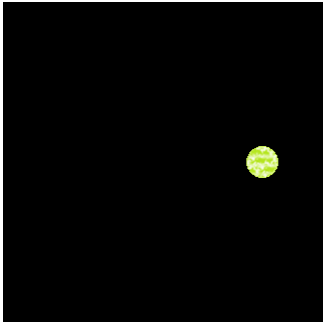
\includegraphics[scale=1]{frontend/prototype-0.png}
	\centering
	\caption{Erster Prototyp}
	\label{figx}
\end{figure}
\newpage
\section{Analyse - Steuerung}
\begin{quote}
	\href{https://github.com/Transport-Protocol/MBC-Ping-Pong/issues/11}{Analyse - Steuerung \#11}
	\newline
	\textit{Die Steuerung des Spiels erfolgt über das Handydisplay. Jedes Handy ist unterschiedlich groß, zudem sollte der Schläger nicht springen können.}
\end{quote}
Es zu analysieren wie sich verschiedene Auflösungen und verschiedene Pixeldichten auf das Spielgefühl auswirken können.
Denkbar ist das Geräte mit einer geringen Pixeldichte gegenüber Spielern mit einer hohen Pixeldichte im Vorteil sind da aus Geräten mit einer hohen Pixeldichte sehr viel kleinere Gesten zur Steuerung ausreichen.
\newline
\textbf{Zielsetzung dieser Analyse}
\begin{enumerate}
	\item
	      \textbf{Feststellung} Es soll festgestellt werden in wie weit sich ein Unterschied der Pixeldichte auf die Spielweise auswirken kann.
	\item
	      \textbf{Behandlung} Es soll geprüft werden ob sich eine mögliche Unfairness beheben lässt und ein mögliches Konzept erstellt werden.
\end{enumerate}
\subsection{Feststellung der Auswirkung verschiedener Pixeldichten}
Je nachdem wie die Steuerung implementiert wird die Pixeldichte eines Steuergerätes mehr oder weniger Einfluss auf das Spiel haben. Das birgt die Gefahr das Spieler mit einem Gerät mit einer geringen Pixeldichte gegenüber einem Spieler mit einem Gerät mit hoher Pixeldichte im Nachteil ist da er wesentlich stärkere Bewegungen auf der Touchfläche ausführen muss.
Theoretisch kann dies dazu führen das Spieler auf einem Tablet mit niedriger Auflösung immer im Nachteil zu Hochauflösenden Smartphones sind.
Laut der Android Spezifikation muss die Pixeldichte von Android Geräten mindestens 100 dpi betragen. Ferner sind in den Spezifikationen Pixeldichten bis zu 640dpi (xxxhdpi) definiert. Geräte mit 640dpi wären Geräten mit 100dpi um 640\% überlegen.
\paragraph{} Angenommen die Schläger würden 1:1 um den Pixelabstand der Controller bewegt werden und das Spielfeld habe eine Höhe von 400 Pixeln.
Auf einem Gerät mit 100dpi müsste der Spieler über eine Stecke von 4 cm streichen müssen um den Schläger von einem Ende zum anderen zu bewegen. Auf einem Gerät mit 640dpi müsste der Spieler nur über eine Stecke von unter einem Zentimeter streichen.
\subsection{Behandeln verschiedener Pixeldichten}
\paragraph{Ermitteln von der DPI im Browser}
\mbox{}\\
Es wird nach vorhanden Lösungen zum erkennen der Pixeldichte in PPI bzw DPI gesucht.
Die gefundenen Beispiele werden dann mit verschiedenen Geräten getestet und die Ergebnisse mit den tatsächlichen DPI verglichen.
\newline\textbf{Die Testgeräte}
\begin{enumerate}
	\item \begin{tabular}{cc}
	      Name & PC Monitor\\
	      Diagonale & 23.6zoll\\
	      Auflösung & 1920*1080\\
	      Pixeldichte & 93 DPI\\
	\end{tabular}
	\item \begin{tabular}{cc}
	      Name & Samsung Galaxy S4\\
	      Diagonale & 4.99zoll\\
	      Auflösung & 1920*1080\\
	      Pixeldichte & 441 DPI\\
	\end{tabular}
	\item \begin{tabular}{cc}
	      Name & Samsung Galaxy Tab A\\
	      Diagonale & 9.7zoll\\
	      Auflösung & 1024*768\\
	      Pixeldichte & 132 DPI\\
	\end{tabular}
\end{enumerate}
\newpage
\begin{itemize}
	\item
	      \textbf{http://www.infobyip.com/detectmonitordpi.php} Eine Website zur Ermittlung der DPI. Es wird ein Quadrat per CSS auf eine bestimmte Größe, zum Beispiel 1 Zoll, formatiert und dann die Größe in Pixeln ausgelesen. Auf diese Weise lässt sich ein DPI wert berechnen.
	      \newline
	      Tests:
	      %\begin{enumerate}
	      \begin{tabular}{ccc}
	      	                     & Erwarteter Wert & Ermittelter Wert           \\
	      	PC Monitor 1         &                 &                            \\
	      	Pixeldichte          & 93 DPI          & \colorbox{red!30}{96 DPI}  \\
	      	Größe des Feldes     & 8 cm            & \colorbox{red!30}{8.2 cm}  \\
	      	                     &                 &                            \\
	      	Samsung Galaxy S4    &                 &                            \\
	      	Pixeldichte          & 441 DPI         & \colorbox{red!30}{288 DPI} \\
	      	Größe des Feldes     & 8 cm            & \colorbox{red!30}{1.8 cm}  \\
	      	                     &                 &                            \\
	      	Samsung Galaxy Tab A &                 &                            \\
	      	Pixeldichte          & 132 DPI         & \colorbox{red!30}{96 DPI}  \\
	      	Größe des Feldes     & 8 cm            & \colorbox{red!30}{5.7 cm}  \\
	      \end{tabular}
	      %\end{enumerate}
	      Getestet wurde jeweils mit Firefox \& Chrome, der PC Monitor wurde auch noch mit dem Edge Browser getestet. Die Ergebnisse waren allesamt für das Gerät identisch.
	      \newline
	      \textbf{Ergebnis:} Die DPI wurden nicht korrekt erkannt. Die Werte weichen auf dem Mobiltelefon um bis zu \underline{77.5\%} ab.
\end{itemize}
\newpage
\paragraph{Verwenden von 'window.devicePixelRatio'}
\mbox{}\\
Die Eigenschaft \textit{window.devicePixelRatio} gibt das Verhältnis der Größe der physikalischen Pixel des aktuellen Displays zu der Größe der Geräteunabhängigen-Pixel (\textit{device independent pixels(dips)}) wieder.
\begin{displaymath}
	window.devicePixelRatio = physical pixels / dips 
\end{displaymath}

Es wird vor allem dafür genutzt um eine Einheitliche Darstellung von Webinhalten auf verschiedenen Displaygrößen zu erreichen.
\newline
Die Methode klingt sehr vielversprechend, also entschied ich einen Test zu erstellen. Meine Idee ist es ein Quadrat zeichnen zu lassen bei dem die Größe abhängig von dem devicePixelRatio ist und dann die Seitenlänge auf dem Display zu messen.
Mein verwendeter Code:
\begin{lstlisting}
var c=document.getElementById("myCanvas");
var ctx=c.getContext("2d");
var w = 100*window.devicePixelRatio;
ctx.rect(20,20,w,w);
ctx.fillText(w,30,30); 
ctx.stroke(); 
\end{lstlisting}

\textbf{Tests:}
\newline
\begin{tabular}{ccc}
	Gerät                  & DevicePixelRatio & Größe TestQuadrat   \\
	PC Monitor 23.6"       & 1.0              & 2.7 cm              \\
	Samsung Galaxy S4      & 3.0              & 1.9 cm              \\
	Samsung Galaxy Tab A   & 1.0              & 1.5 cm              \\
	Samsung Galaxy S3 Neo  & 2.0              & 1.3 cm              \\
	Samsung Galaxy S5 mini & 2.0              & 1.1 cm              \\
	Samsung Galaxy S7 edge & 4.0              & >4 cm               \\
\end{tabular}
\paragraph{Ergebnis:}
\mbox{}\\
Das Ergebnis der Tests ist leider ernüchternd. Die ersten Geräte zeigten das Quardrat allesamt in einer ähnlichen Größe. Doch auf weiteren Testgeräten zeigte sich das die Größe sehr stark variierte. Auf dem Samsung Galaxy S7 edge war das Quadrat sogar sehr viel größer als der vordefinierte Bereich.
\newpage
\paragraph{Suche nach Alternativen zu DevicePixelRatio}
\mbox{}\\
An vielen Stellen habe ich gelesen das der DevicePixelRatio sehr häufig gerundet wird. Dies fiel ebenfalls bei den Testgeräten auf.
\newline
Also kam mir die Idee eine eigene Version der Funktion zu schreiben. In Javascript kann man mit folgender Funktion testen ob ein bestimmter DevicePixelRatio unterstützt wird.
\begin{lstlisting}
if (window.matchMedia('(-webkit-min-device-pixel-ratio: 1)').matches) 
\end{lstlisting}
Meine Idee war es den gewünschten Wert der Funktion schrittweise zu erhöhen und den zuletzt akzeptierten Wert zurückzugeben.
\newline
Daraus ergab sich folgende Funktion:
\begin{lstlisting}
function getDPR() {
    var numb = 1.0;
    while(window.matchMedia(
    	'(-webkit-min-device-pixel-ratio: ' + numb + ')'
    	).matches) {
        	numb += 0.1;
    }
    return numb - 0.1;
}
\end{lstlisting}
Leider ergaben die Test mit dieser Funktion keine nennenswerte Ergebnisse weswegen ich auf eine Auflistung und Auswertung der Ergebnisse in diesem Falle verzichte.
\paragraph{Verwendung der CSS3 MediaQuery Eigenschaften}
\mbox{}\\
Mit CSS3 lassen sich verschiedene Fälle für verschiedene Auflösungen definieren.
\begin{figure}[ht]
	\centering
	\begin{lstlisting}
@media (resolution: 96dpi) { /* Exakt 96 Bildpunkte pro Zoll */ }
@media (min-resolution: 200dpcm) { /* Mindestens 200 Punkte pro cm */ }
@media (max-resolution: 300dpi) { /* Maximal 300 Punkte pro Zoll */ }
	\end{lstlisting}
	\caption{Quelle: https:\/\/wiki.selfhtml.org\/wiki\/CSS\/Media\_Queries}
	\label{figx}
\end{figure}
\newline
Hiermit ist es möglich für die verschiedenen Pixeldichten die Kontrollfelder anzupassen. Allerdings werden die Pixeldichten der Geräte nicht immer richtig erkannt. Es 
\newpage
\subsection{Ergebnis der Analyse}
Es gibt leider keine Möglichkeit eine Webapp mit exakten physikalischen Größen zu gestalten.
\paragraph{Gestaltung per CSS Einheiten} In CSS besteht die Möglichkeit Größen in CM oder Zoll zu definieren. Leider entsprechen die Werte auf Mobilen Endgeräten nicht den gewünschten Werten.
\paragraph{Gestaltung mit Device Pixel Ratio} Die Gestaltung per DevicePixelRatio erscheint wesentlich genauer als die Gestaltung mit CSS Längenangaben allerdings ist auch diese Lösung sehr ungenau und lässt sich nicht einheitlich nutzen. 
\paragraph{Gestaltung der Steuerung} Man könnte die Steuerung so definieren das ein Vorteil der Pixeldichte sich nicht zu sehr auf das Spiel auswirkt. Beispielsweise Kann man eine Maximalgeschwindigkeit der Schläger so definieren das sie auch auf Geräten mit geringer Pixeldichte leicht erreicht werden kann. Dadurch sind allerdings möglicherweise Geräte mit hoher Pixeldichte im Nachteil da man für kurze Bewegungen nur noch minimale Bewegungen auf dem Bildschirm durchführen dürfte.
\newline
Denkbar wäre auch eine Steuerung mit fester Bewegungsgeschwindigkeit sodass nur noch die Richtung der Schläger durch die Controller geregelt wird. Diese Art Steuerung verspricht allerdings nicht viel Spaß oder Reaktionsmöglichkeiten der Spieler.
\newline
\newline
\textbf{Lösungsmöglichkeit:}
\paragraph{Verrechnung der Information zur Pixeldichte} 
\mbox{}\\
Mit den CSS3 Media Queries ist es zumindest ansatzweise Möglich die Pixeldichte der Geräte zu erkennen. Allerdings sich auch sie sehr ungenau und keinesfalls verlässlich.
\newline
Zur fairen Gestaltung der Touchfelder sollten wir die Media Queries bzw den DevicePixelRatio verwenden um zwischen Geräten mit hoher und geringerer Pixeldichte unterscheiden.
\newline
Beispielsweise indem wir den PixelRatio mit der zurückgelegten Stecke in Pixeln verrechnen.
\begin{lstlisting}
movement = screenDistance / window.devicePixelRatio;
\end{lstlisting}
Somit werden Geräte mit einem PixelRatio von 1 nicht benachteiligt. Außerdem hat dies zur Folge das Spieler auf einem Gerät mit einem hohen PixelRatio ihre Schläger nicht unnötig schnell bewegen wenn sie zum Beispiel nur kurze Bewegungen erreichen wollen.
\newline 
Ein Problem bleibt jedoch, der PixelRatio ist nicht sehr genau. Um ein Gefühl für die Auswirkungen zu bekommen müssen wir mehrere Testgeräte für die Steuerung verwenden.
\subsection{Flüssige Bewegung}
Um eine flüssige Bewegung zu garantieren sollten wir uns auf einige Eigenschaften der Steuerung festlegen.
\paragraph{Anforderung: Bildschirmposition != Schlägerposition}
\mbox{}\\
Die Schläger sollen in Abhängigkeit einer Bewegung, also einer Positionsänderung auf dem Bildschirm bewegt werden. Das bedeutet für uns das wir die Information der Controller nicht als Absolute Positionen sehen sondern eher die Änderung während einer Geste betrachten.
\newline
Hierfür sei folgendes Festgelegt:
\begin{itemize}
	\item 
	      \textbf{Beginn der Geste:} Eine Geste beginnt mit dem Berühren des Touchfeldes. Die Startposition wird ermittelt und in einer Variable gespeichert.
	\item
	      \textbf{Während der Geste:} Während der Finger sich auf dem Touchfeld bewegt wird die neue Position des Fingers ausgewertet. Die neue Position wird von der alten Position abgezogen wodurch sich eine Differenz ergibt. Diese wird dann mit dem PixelRatio verrechnet und an das Spiel (DisplayPeer) geschickt.
	      \newline
	      Der ganze Prozess sollte alle 40ms neu gestartet werden.
	\item
	      \textbf{Ende einer Geste: } Eine Geste endet sobald das Touchfeld nicht mehr berührt wird. Die aktuelle Änderung der position wird auf 0 gesetzt.
\end{itemize}
Wenn der Controller nicht mehr berührt wird so darf sich der Schläger nicht weiter bewegen. Der Controller braucht in diesem Zustand dem Spiel keine Infos übermitteln.
\newline
Moderne Mobiltelefone haben wesentlich höhere Auflösungen als unser Spielfeld groß sein wird. Aus diesem Grund sollte die Bewegung auf einem Maximumwert begrenzt werden.
\newline 
Maximal sollte sich ein Schläger über die gesamte Spielfläche in einem Zyklus bewegen können. Es ist denkbar das wir den Wert später nach unten korrigieren müssen um ein gutes Spielgefühl schaffen zu können.
